\section[M4: Xtend]{M4: Xtend - Java Quellcode Generierung}
\begin{frame}{Code-Generierung mit Xtend}
	\centering
	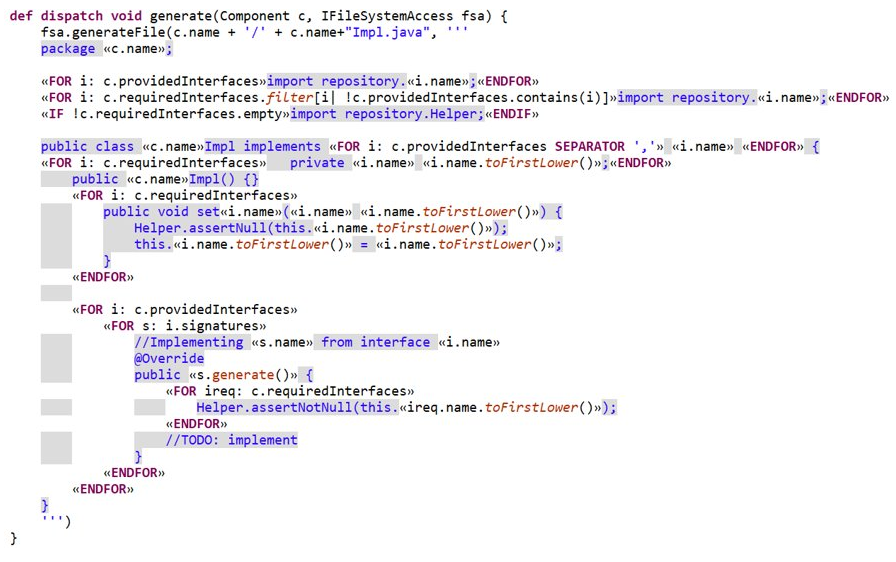
\includegraphics[height=60mm]{figures/xtend.png}
\end{frame}

\begin{frame}{Problem mit Xtend und OCL}
	\begin{enumerate}
		\item Xtend-Validator kann OCL Constraints nicht einlesen und validieren
		\item Vorrübergehende Lösung = \textit{NullValidator}
	\end{enumerate}
	\centering
	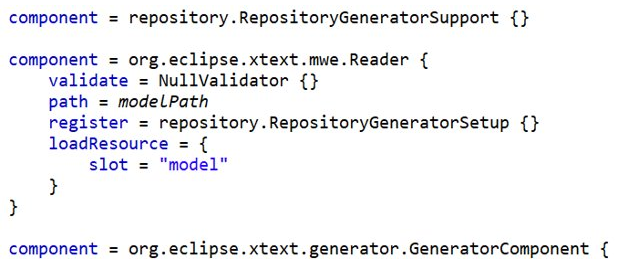
\includegraphics[height=40mm]{figures/xtend-validator.png}
	\begin{itemize}
		\item Model kann eingelesen und Java generiert werden
		\item auch nicht-valide Modelle weredn akzeptiert und transpiliert
	\end{itemize}
\end{frame}